\chapter{System Requirements and High-Level Architecture}

\section{Introduction}
Engineering a resilient, distributed, two-sided marketplace requires structured requirements specification and formal architectural modeling. This chapter establishes the Software Requirements Specification (SRS), non-functional constraints, 3-tier distributed architecture, UML sequence interactions, and operational environments for StayMart.

\section{Software Requirements Specification (SRS)}

\subsection{User Personas and Actor Hierarchy}
StayMart delineates four primary actor classifications interacting within the platform ecosystem:
\begin{enumerate}
    \item \textbf{Guest User:} Unauthenticated visitor with read-only access to approved listings, regional filters, and public categories.
    \item \textbf{Verified Tenant / Buyer:} Registered user authenticated via JWT bearer token with privileges to book rooms, order items, save wishlists, and initiate peer chat.
    \item \textbf{Property Host / Seller:} Authenticated listing author managing room inventories, pricing tiers, deposits, condition notes, and order state transitions.
    \item \textbf{Platform Administrator:} Privileged operator (\texttt{ROLE\_ADMIN}) governing pre-publication moderation, auditing accounts, and viewing telemetry.
\end{enumerate}

\begin{figure}[htbp]
    \centering
    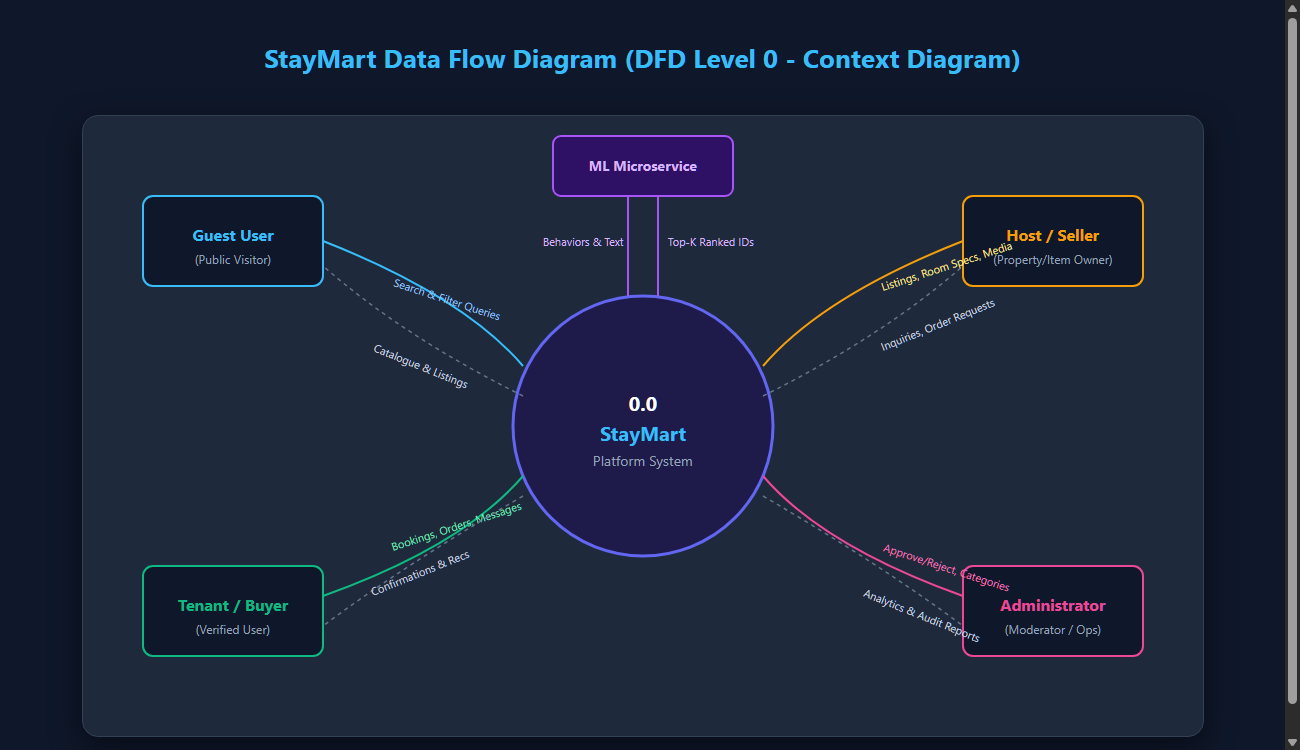
\includegraphics[width=0.92\textwidth]{diagrams/dfd_level0.png}
    \caption{Data Flow Diagram Level 0 (Context Level Diagram) for the StayMart System}
    \label{fig:dfd0}
\end{figure}

\subsection{Functional Requirements (FR)}
The functional scope is structured into eight core modules summarized in Table \ref{tab:functional_reqs}.

\begin{table}[htbp]
\centering
\caption{Comprehensive Functional Requirements Specification}
\label{tab:functional_reqs}
\footnotesize
\begin{tabularx}{\textwidth}{lp{3.8cm}X}
\toprule
\textbf{Module ID} & \textbf{Module Name} & \textbf{Functional Description and Expected System Behavior} \\
\midrule
\textbf{FR-01} & Authentication \& RBAC & Email uniqueness check, BCrypt password hashing ($cost=10$), JWT generation (HMAC-SHA256, 24h expiration), role enforcement (\texttt{ROLE\_USER}, \texttt{ROLE\_ADMIN}). \\
\textbf{FR-02} & Accommodation Mgmt & CRUD operations for 6 property types with amenities, room inventories, security deposits, address mapping, and multi-image JSON payloads. \\
\textbf{FR-03} & Room-Level Inventory & Multi-unit property association with discrete rooms (Single, Double, Triple, Dorm) specifying room number, floor, rent, and vacancy toggles. \\
\textbf{FR-04} & Product Marketplace & CRUD operations for student goods across 10 categories (Sell vs. Rent), capturing condition grading (Brand New to Fair) and wear specifications. \\
\textbf{FR-05} & Lifecycle Transactions & End-to-end booking state machine (\texttt{PENDING} $\rightarrow$ \texttt{CONFIRMED} $\rightarrow$ \texttt{COMPLETED} / \texttt{CANCELLED}) and order decrement workflows. \\
\textbf{FR-06} & Peer-to-Peer Messaging & Real-time bilateral chat between buyers/tenants and sellers/hosts with unread badges and listing context injection. \\
\textbf{FR-07} & ML Recommendations & Asynchronous microservice integration delivering personalized listings, similar item carousels, and top-rated rankings based on telemetry. \\
\textbf{FR-08} & Admin Governance & Pre-publication moderation queue, account deactivation rules, location/category CRUD, and telemetry chart aggregation. \\
\bottomrule
\end{tabularx}
\end{table}

\subsection{Non-Functional Requirements (NFR)}
\begin{enumerate}
    \item \textbf{Performance (NFR-01):} Core read APIs must respond in $t_{\text{resp}} < 50\text{ ms}$; recommendation endpoints must return within $t_{\text{ml}} < 120\text{ ms}$.
    \item \textbf{Security (NFR-02):} BCrypt password hashing, Spring Data JPA parameterized queries preventing SQL injection, output sanitization via \texttt{escapeHtml()}, and stateless JWT tokens.
    \item \textbf{Data Integrity (NFR-03):} Inventory modifications execute within isolated Spring \texttt{@Transactional} boundaries adhering to ACID guarantees.
    \item \textbf{Decoupling (NFR-04):} The ML microservice is isolated from the transactional Spring Boot core, enabling independent horizontal scaling.
    \item \textbf{Usability (NFR-05):} Responsive layouts from 320px (mobile) to 1280px+ (desktop) adhering to WCAG AAA contrast and zero horizontal overflow.
\end{enumerate}

\section{High-Level 3-Tier Distributed Architecture}
StayMart partitions responsibilities across three decoupled distributed tiers:
\begin{enumerate}
    \item \textbf{Presentation Tier (Client Portal):} Vanilla ES6 JavaScript, HTML5, and CSS3 communicating asynchronously over HTTPS via JSON payloads. Stateless JWT tokens are stored in browser storage and transmitted via \texttt{Authorization: Bearer <JWT>} headers.
    \item \textbf{Business Tier (Spring Boot 3.3 Core):} Executing on Eclipse Temurin OpenJDK 17 LTS, this tier implements a Controller-Service-Repository pattern across 16 REST resource controllers, custom \texttt{JwtAuthenticationFilter}, transactional service handlers, and 12 Spring Data JPA repositories.
    \item \textbf{Persistence and ML Tier:} MySQL 8.0 InnoDB provides ACID persistence across 12 normalized tables. A companion Python 3.11 / Flask WSGI service executes TF-IDF vectorization and serves similarity predictions via REST endpoints.
\end{enumerate}

\section{UML Behavioral Modeling: Sequence Diagrams}
Figure \ref{fig:seq_booking} details the complete lifecycle of an accommodation booking transaction across the three tiers.

\begin{figure}[htbp]
    \centering
    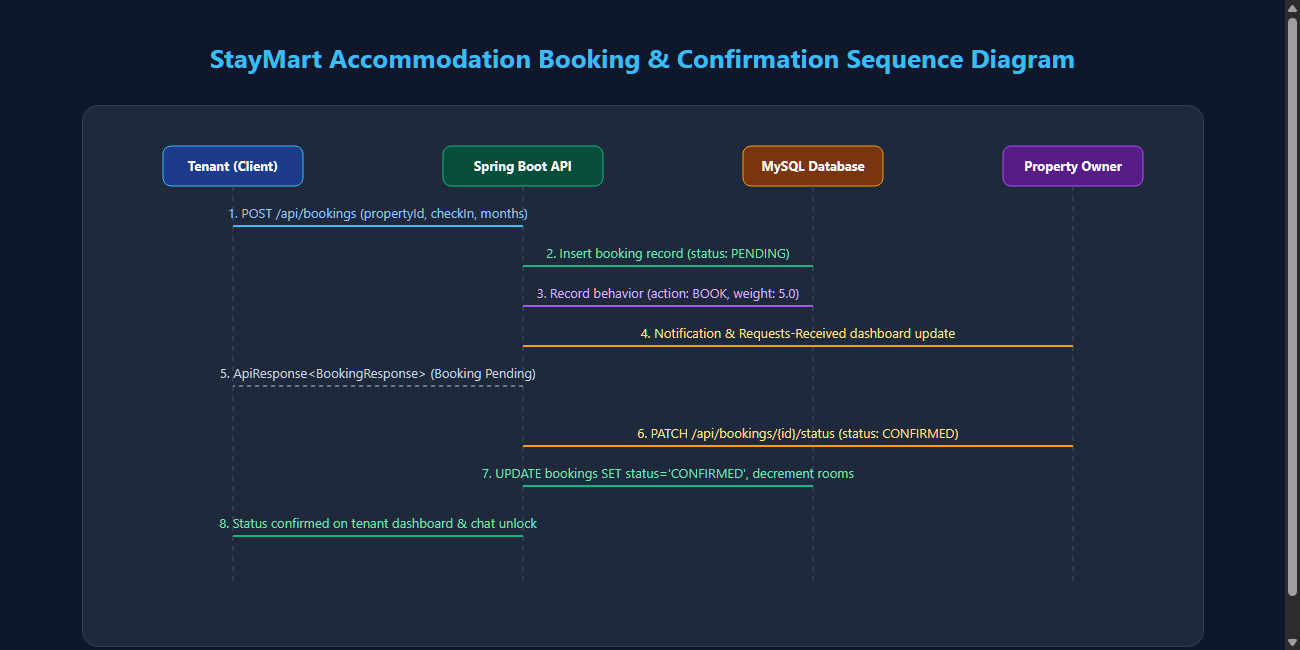
\includegraphics[width=0.92\textwidth]{diagrams/seq_booking.png}
    \caption{UML Sequence Diagram: Accommodation Booking and Confirmation Flow}
    \label{fig:seq_booking}
\end{figure}

The sequence executes through eight calculated stages: (1) tenant submits \texttt{POST /api/bookings}; (2) controller validates JWT and room capacity; (3) service persists booking as \texttt{PENDING}; (4) \texttt{BehaviorService} synchronously logs telemetry ($\text{weight}=5.0$); (5) API returns \texttt{ApiResponse<BookingResponse>} (201 Created); (6) host is alerted via requests dashboard; (7) host submits \texttt{PATCH /api/bookings/\{id\}/status?status=CONFIRMED}; (8) status transitions to \texttt{CONFIRMED}, available bed count decrements, and direct chat is unlocked.

\section{Hardware and Software Operational Environments}
Table \ref{tab:environment_specs} summarizes the operational specifications required to host and execute the StayMart platform.

\begin{table}[htbp]
\centering
\caption{System Hardware and Software Operational Specifications}
\label{tab:environment_specs}
\footnotesize
\begin{tabularx}{\textwidth}{lp{4.2cm}X}
\toprule
\textbf{Layer} & \textbf{Specification Parameter} & \textbf{Recommended Value / Deployment Minimum} \\
\midrule
\multirow{4}{*}{\textbf{Hardware}} & CPU Architecture & x86\_64 (AMD64) or ARM64 (AWS Graviton), 4+ Cores \\
& RAM & 8 GB Minimum (16 GB Recommended for Dockerized Prod) \\
& Storage & 50 GB NVMe SSD (Persistent MySQL Volume + Uploads) \\
& Network & 100 Mbps Full-Duplex Network Interface Card \\
\midrule
\multirow{4}{*}{\textbf{Backend}} & Java Runtime & Eclipse Temurin OpenJDK 17 LTS \\
& Framework & Spring Boot 3.3.5 (Spring Framework 6.1.14) \\
& Build Tool & Apache Maven 3.9.9+ \\
& Embedded Servlet & Apache Tomcat 10.1.31 (HTTP Port 8080) \\
\midrule
\multirow{4}{*}{\textbf{ML Service}} & Python Interpreter & Python 3.11.9+ \\
& Scientific Packages & scikit-learn 1.3.0, pandas 2.0.3, numpy 1.24.4 \\
& Web Framework & Flask 2.3.3 with Flask-CORS 4.0.0 \\
& Production WSGI & Threaded runtime (development) / Gunicorn (Docker) \\
\midrule
\multirow{3}{*}{\textbf{Database}} & Relational Database & MySQL Community Server 8.0.35+ \\
& Storage Engine & InnoDB with UTF8MB4 Character Set \\
& Connection Pool & HikariCP (Maximum Pool Size: 10 Connections) \\
\midrule
\multirow{3}{*}{\textbf{Frontend}} & Client Technologies & Semantic HTML5, CSS3 Custom Properties, JavaScript ES6+ \\
& Visual Rendering & Chart.js 4.4+ (Dashboard Telemetry) \\
& Static Host / Server & Multi-threaded Python server (Dev) / Vercel Edge CDN \\
\bottomrule
\end{tabularx}
\end{table}

\section{Summary}
This chapter formalised the SRS for StayMart across four personas, eight functional modules, and strict performance and security constraints. Through UML sequence modeling and 3-tier decoupling, the interaction contracts were established. The next chapter explores database relational modeling and normalization analysis.
